Data for our preliminary results were collected using Google Forms. The
prototype would direct the user to take an entry survey, guide them through the
features, and then finish with an exit survey. The two surveys contained the
following questions:

\begin{center}
  \begin{tabular}{|l|p{0.6\linewidth}|}
    \hline
    \multicolumn{2}{|c|}{\Large \textbf{Entry Survey}}\\
    \hline
    \multirow{6}{*}{\textbf{Demographics}}
 & Name \\ \cline{2-2}
 & Age \\\cline{2-2}
 & Gender \\\cline{2-2}
 & Education \\\cline{2-2}
 & Major \\\cline{2-2}
 & Primary OS \\
    \hline
    \multirow{6}{*}{\textbf{Familiarity}}
 & I think the command line is easy to use. \\ \cline{2-2}
 & I think the command line is more usable than a GUI. \\ \cline{2-2}
 & I feel comfortable using the shell. \\ \cline{2-2}
 & I prefer command line tools to GUI tools.\\ \cline{2-2}
 & I think I would prefer the shell if I understood it better (or already
   do).\\ \cline{2-2}
 & I think the shell is easy to learn.\\
    \hline
    \multirow{4}{*}{\textbf{Proficiency}}
 & I use piping and redirection. \\ \cline{2-2}
 & I use control structures in the shell.\\ \cline{2-2}
 & I use wild cards in the shell.\\
    \hline
    \multirow{5}{*}{\textbf{Confidence}}
 & When presented with a problem, I know the commands to use. \\ \cline{2-2}
 & I feel that learning how to use new commands is easy. \\ \cline{2-2}
 & I use a wide array of commands. \\ \cline{2-2}
 & I feel that I have sufficient knowledge of the shell for what I need. \\
    \hline
    \multirow{1}{*}{\textbf{Qualitative}} & Explain what tasks you commonly carry
                                            out on in the shell.\\
    \hline
  \end{tabular}
\end{center}

\begin{center}
  \begin{tabular}{|l|p{0.6\linewidth}|}
    \hline \multicolumn{2}{|c|}{\textbf{\Large Exit Survey}} \\ \hline
    \multirow{4}{*}{\textbf{Usability}}
    & This system would improve my usage of the shell. \\ \cline{2-2}
    & This system would help me solve problems in the shell. \\ \cline{2-2}
    & This system is more usable than a traditional shell. \\ \cline{2-2}
    & I find the interface of the system inviting and usable. \\
    \hline
    \multirow{3}{*}{\textbf{Educational Value}}
    & This system would teach me commands in a more effective way than the
      status quo. \\ \cline{2-2}
    & This system would help me perform automation that I would not make on my
      own.\\ \cline{2-2}
    & Using this system would improve my understanding of all shells.\\
    \hline
    \multirow{3}{*}{\textbf{Intention}}
    & I would prefer this to the normal shell experience. \\ \cline{2-2}
    & I would use this system in the future. \\ \cline{2-2}
    & I would suggest this system to others. \\
    \hline
    \multirow{2}{*}{\textbf{Qualitative Critique}}
    & What did you like most about the system?  \\ \cline{2-2}
    & What do you think needs the most improvements? \\
    \hline
  \end{tabular}
\end{center}

In between these surveys we presented a demo of our system. There were 28 total
respondents to the survey, only 15 of whom completed both the entry and the exit
surveys.

\subsection{Data Analysis}

Data analysis was carried out using scientific computing libraries provided by
the Julia and Python programming languages. A cursory data analysis was also
provided by Google Forms, which gave a basic initial overview of the responses
to each question.

The first thing we wanted to do was understand the demographics of our survey.
The questions of age and gender did not show enough diversity to be very
statistically useful \-- almost all of the respondents were males between the
ages of 18 and 24. Education level showed a more promisingly even distribution,
and while the question of primary operating system is skewed in favor of Linux
(clearly indicating more selection bias), users of other OSes still have a
decent representation.

\begin{figure}[ht]
  \centering
  \begin{subfigure}[b]{0.45\textwidth}
    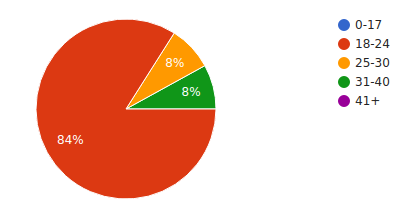
\includegraphics[width=\textwidth]{figures/stats/age.png}
    \caption{Age}
    \label{fig:age}
  \end{subfigure}
  \quad
  \begin{subfigure}[b]{0.45\textwidth}
    \label{fig:gender}
    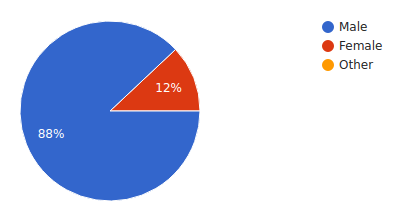
\includegraphics[width=\textwidth]{figures/stats/gender.png}
    \caption{Gender}
  \end{subfigure}

  \begin{subfigure}[b]{0.45\textwidth}
    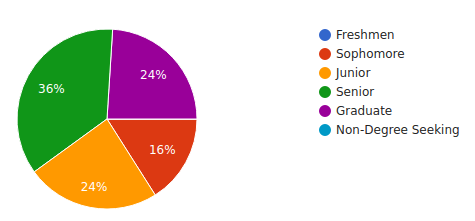
\includegraphics[width=\textwidth]{figures/stats/edu.png}
    \caption{Education}
    \label{fig:edu}
  \end{subfigure}
  \quad
  \begin{subfigure}[b]{0.45\textwidth}
    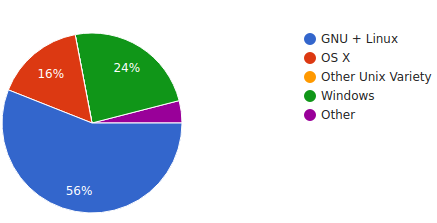
\includegraphics[width=\textwidth]{figures/stats/os.png}
    \caption{Primary OS}
    \label{fig:OS}
  \end{subfigure}
  \caption{Main demographic information for survey base}
\end{figure}

Our entry survey also includes questions pertaining to the users' abilities when
using the terminal. Figure \ref{fig:skillz} shows a histogram representing a
simple additive ranking of the participants self-reported abilities. The
majority of our users claimed to be more experienced with the shell, which is
very unfortunate because that does not match at all with the target audience we
hoped to be gathering feedback from. There was still some novice representation
in the data, so it was still possible to correlate the survey responses with
skill levels.

\begin{figure}[H]
  \centering
  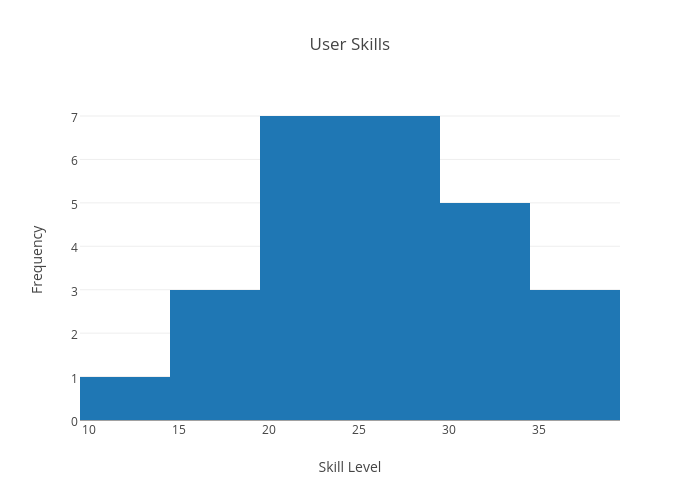
\includegraphics[width=0.6\textwidth]{figures/stats/user-skills.png}
  \caption{Histogram of the relative skill levels of our users. Note the larger
    right tail.}
  \label{fig:skillz}
\end{figure}

We wanted to learn as much as possible from our limited data, so we calculated
the Pearson correlation coefficient between the sets of responses for
\emph{every} pair of survey questions. This allowed us to detect every single
interrelationship between the entry and exit surveys that could be considered at
all interesting. The first major surprise to come out of this exhaustive
approach was that there were no significant correlations at all for \emph{any}
of the demographic questions\footnote{The most significant demographic was
  education level, but it was still not associated with anything with a
  $p$-value less $0.10$!}. The questions like age and gender and level of
education don't allow us to draw any meaningful conclusions, however there are
still interesting connections between the questions themselves.

\begin{figure}[ht]
  \centering
  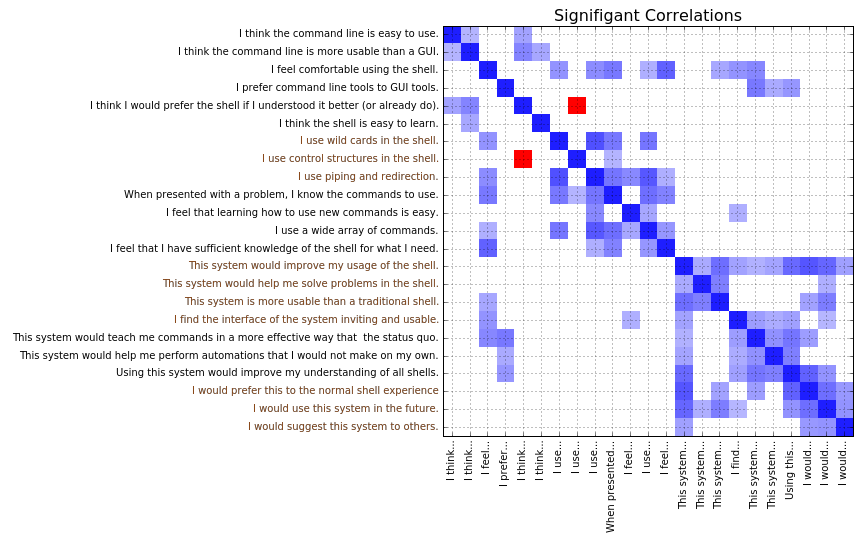
\includegraphics[width=\textwidth]{figures/stats/sig.png}
  \caption{A matrix highlighting the Pearson correlations between each pair of
    survey questions for which the $p$-value was $< 0.05$. Darker squares
    indicate stronger correlations.}
  \label{fig:pvalplot}
\end{figure}

Figure \ref{fig:pvalplot} shows a heat map of the statistically significant
Pearson correlations in the responses to our survey. Our entry survey contained
groups of questions intended to determine a user's familiarity, proficiency, and
confidence with the shell. Looking at the Pearson graph, we can briefly examine
how well-correlated the individual questions are to their groups. The
familiarity group, in the top left corner, is the least self-correlated of these
three groups. The following two \-- proficiency and confidence \-- show more
self correlation, with most of questions correlated to at least half of their
own groups.

Our exit survey was broken into three question groups designed for probing a
user's opinion on the usability of the shell, it's educational potential, and
their overall experience with it. Looking at the bottom half of the Pearson
graph, it can be seen that these question groups are very well self-correlated.

The Pearson graph shows a few patterns of interest. Note the question from our
entry survey, ``I feel comfortable using the shell''. This question is
correlated with parts of the usability and education question groups on the exit
survey; it's most strongly correlated with the entry survey question "I feel
that I have sufficient knowledge of the shell for what I need."

The surveys have a single negative correlation of significance. It's between two
questions on the entry survey: ``I use control structures in the shell'' and ``I
think I would prefer the shell if I understood it''.

\begin{figure}[H]
  \centering
  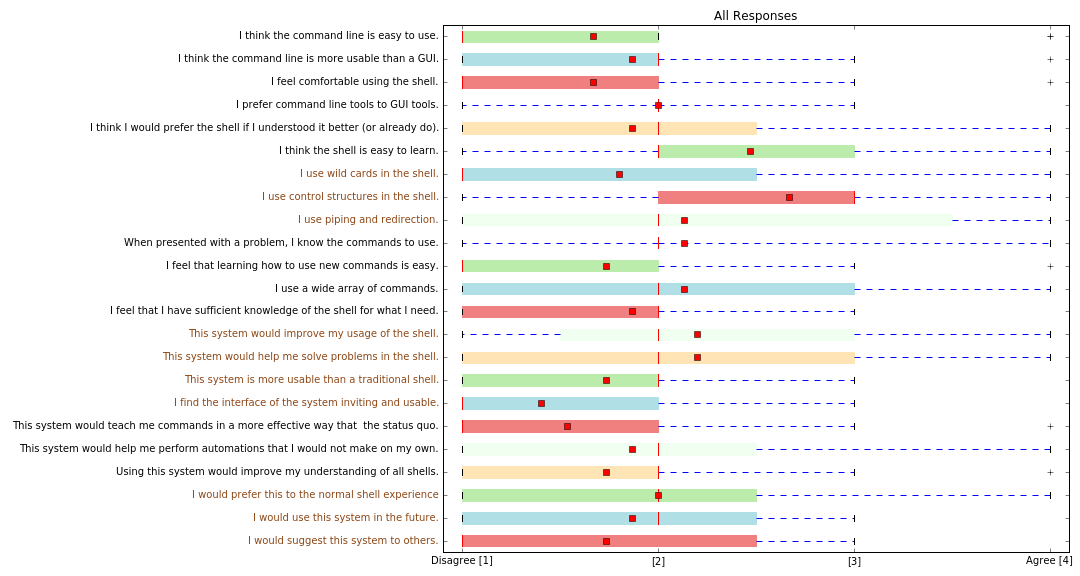
\includegraphics[width=\textwidth]{figures/stats/all.png}
  \caption{Data is free}
  \label{fig:alldata}
\end{figure}

In Figure \ref{fig:alldata} can be seen an overview of our full responses. There
were no correlations of significance between users' education levels and their
responses to any of the questions, so we choose to analyze the responses as a
single group. On the entry survey most users reported low comfort with shell
usage and a preference for GUI tools. Almost all users use piping and
redirection in the shell; control structure use is less common; most users do
not use wildcards. Within the confidence group most users reported difficulties
with retaining and finding the information they need to complete tasks. Most
users did not feel that they used a wide array of commands.

From the exit survey we conclude that most users disagreed with our prototype
being usable, educational, or overall a pleasant good experience.

\subsection{Qualitative Analysis}
    % 8d. Describe the quantitative/qualitative analysis results with proper
    % statistics test/grounded theory. You should also indicate whether or not the
    % analysis result can support the hypotheses in Section 8.

Our entry and exit surveys each had at least one qualitative response question.
The responses to these can be seen in Appendix
% \ref{fig:fig_data}.
The entry survey asked users what tasks they commonly carried out in the shell.
Seven out of the fifteen responses indicated navigation and file manipulation,
five indicated programming-related tasks, and four indicated searching.

There were two qualitative response questions on the exit survey. The first
asked users what they liked most about the prototype. There is no clear
consensus here \-- users reported liking the GUI elements, the context window, the
undo functionality, the suggested automations, and other disparate features.

The second asked users what they thought needed the most improvement in the
prototype. Three users indicated that more information is needed in the
interface; one wrote: ``More instructions on what the buttons on bottom will do
if pressed would be nice \-- I know the functionality of the buttons isn't
implemented yet, but a small message explaining what the buttons represent and
happens when they are clicked would go a long way.'' Two users reported
confusion with the prototype. Five did not provide an answer or indicated that
they had no suggestions.

%%% Local Variables:
%%% mode: latex
%%% TeX-master: "documentation"
%%% End:
